\documentclass[14pt]{report}

\usepackage{geometry}
\usepackage[utf8]{inputenc}
\usepackage{amsmath}
\usepackage{amsfonts}
\usepackage{amssymb}
\usepackage{graphicx}
\usepackage[utf8]{inputenc}
\usepackage{amsmath}
\usepackage{amsfonts}
\usepackage{amssymb}
\usepackage[shortlabels]{enumitem}
\usepackage{listings}
\usepackage{xcolor}
\usepackage[most]{tcolorbox}
\usepackage{mathtools}
\usepackage{float}
\usepackage[colorlinks=false, linktocpage=true]{hyperref}
\usepackage{enumitem}

\usepackage{booktabs}% http://ctan.org/pkg/booktabs
\newcommand{\tabitem}{~~\llap{\textbullet}~~}
\usepackage{longtable}
 
\usepackage{caption}
\DeclareCaptionType{code}[Code Listing][List of Code Listings] 

\definecolor{codegreen}{rgb}{0,0.6,0}
\definecolor{codegray}{rgb}{0.5,0.5,0.5}
\definecolor{codepurple}{rgb}{0.58,0,0.82}
\definecolor{backcolour}{rgb}{0.95,0.95,0.92}
 
\lstdefinestyle{mystyle}{
    backgroundcolor=\color{backcolour},   
    commentstyle=\color{codegreen},
    keywordstyle=\color{magenta},
    numberstyle=\tiny\color{codegray},
    stringstyle=\color{codepurple},
    basicstyle=\ttfamily\footnotesize,
    breakatwhitespace=false,         
    breaklines=true,                 
    captionpos=b,                    
    keepspaces=true,                 
    numbers=left,                    
    numbersep=5pt,                  
    showspaces=false,                
    showstringspaces=false,
    showtabs=false,                  
    tabsize=2
}
 
\lstset{style=mystyle}

\setlength{\parindent}{0em}
\setlength{\parskip}{1em}

\author{Brian Rashap, Ph.D.}
\title{PHYS 1320 - Calculus-based Physics II}

\geometry{letterpaper, portrait, margin=0.75in}

\begin{document}

\begin{center}
\textbf{Physics 1320 - Calculus-based Physics II \\ Summer 2022 \\ Final Exam}
\end{center}

\textbf{Question 1} (15 pts)



Consider three infinitely long current carrying wires as shown below:
\begin{itemize}
\item Wire 1 is at the origin and carries $3A$ out of the paper.
\item Wire 2 is at coordinates (3cm,0cm) and carries $3A$ into the paper.
\item Wire 3 is at coordinates (3cm,4cm) and carries $3A$ out of the paper.
\end{itemize}

\begin{figure}[H]
\begin{center}
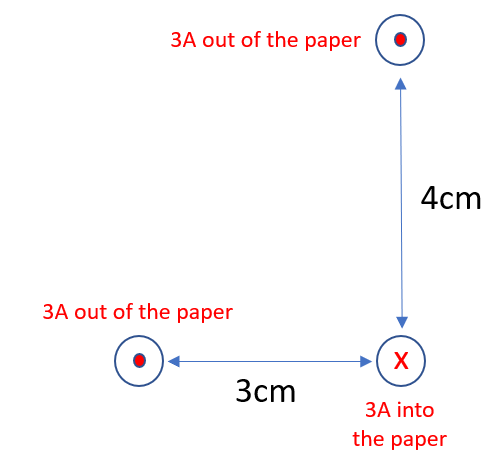
\includegraphics[scale=0.38]{final_1.png}
\end{center}
\end{figure}

What is the Force per unit length (magnitude and direction) exerted on Wire 3?

\textbf{Question 2} (10 pts)

Consider the circuit drawn below

\begin{figure}[H]
\begin{center}
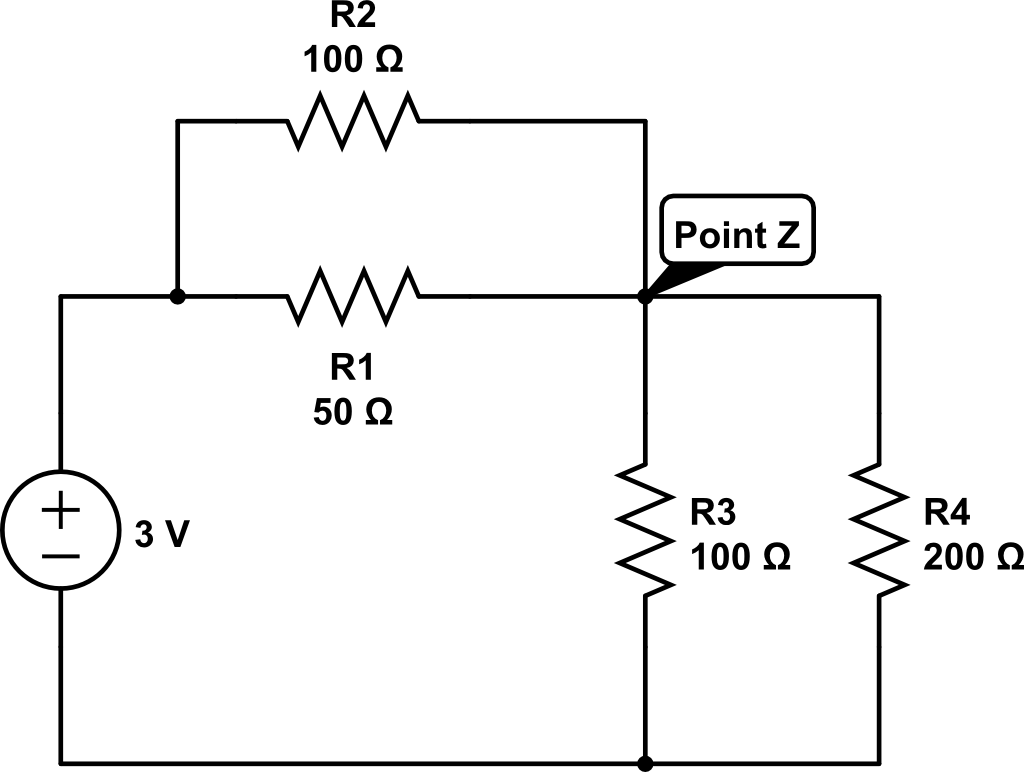
\includegraphics[scale=0.38]{final_2.png}
\end{center}
\end{figure}

\begin{enumerate}[label=\Alph*]
\item What is the equivalent resistance of this circuit?
\item What is the voltage at Point Z?
\item What is the current through resistor R4?
\end{enumerate}

\newpage

\textbf{Question 3} (15 pts)

The LightSail spacecraft has a totally reflective mirror sail that has an area of $32m^2$ and the total spacecraft weight is $5.0kg$. A laser beam is directed at the sail and has an intensity of $13700 \frac{W}{m^2}$ when it reaches the LightSail.

\begin{enumerate}[label=\Alph*]
\item What is the maximum acceleration the LightSail spacecraft can achieve?
\item Assuming the intensity remains constant during the journey, how fast with the LightSail be moving after a year?
\end{enumerate}

\textbf{Question 4} (10 pts)

Recall the relationship that for two parallel plates separated by distance $d$ that $E = \frac{V}{d}$. Consider a proton placed directly between the two plates with voltage of $10.425 kV$. 

\begin{figure}[H]
\begin{center}
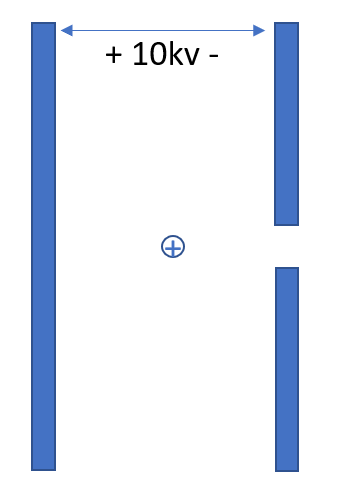
\includegraphics[scale=0.25]{final_4a.png}
\end{center}
\end{figure}

At what speed and in what direction will the proton exit the plates. 

\textbf{Question 5} (15 pts)

Consider the same proton from Problem 4, not traveling with a velocity $\vec{v} = -1*10^6 (\frac{m}{s}) \hat{k}$. It is passing through a chamber with an Electric Field $\vec{E} = -100 (\frac{J}{C}) \hat{j}$ and Magnetic Field $\vec{B} = -0.1 (mT) \hat{i}$.

\begin{figure}[H]
\begin{center}
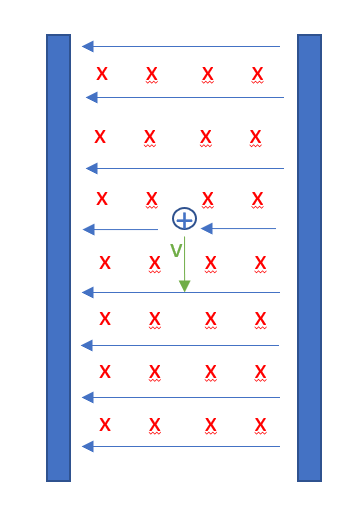
\includegraphics[scale=0.25]{final_4b.png}
\end{center}
\end{figure}

\begin{enumerate}[label=\Alph*]
\item What is the force from the Electric Field ($\vec{F}_E$) experienced by the proton?
\item What is the force from the Magnetic Field ($\vec{F}_B$) experienced by the proton?
\item What is the net (or total) force ($\vec{F}$) experienced by the proton?
\end{enumerate}

\newpage
\textbf{Question 6} (15 pts)

If the proton from Problem 6 now enters a uniform magnetic field $\vec{B} = 10.5 (mT)$ in the directions shown in the diagram below. If the proton enters the origin: point (0,0):

\begin{figure}[H]
\begin{center}
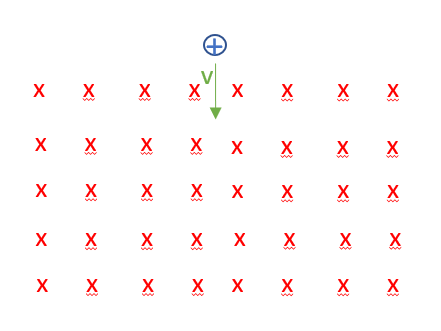
\includegraphics[scale=0.50]{final_4c.png}
\end{center}
\end{figure}

\begin{enumerate}[label=\Alph*]
\item Where does the proton exit the magnetic field?
\item How long does the proton spend in the magnetic field?
\item If we combine the parts from Questions 4,5, and 6, what device do we have?
\end{enumerate} 

\textbf{Question 7} (20 pts)

Consider the following current-carrying conductor with $R_1 = 0.100mm$ and $R_2 = 0.141mm$. Assume the current of $10 mA$ has a uniform current density in the conductor. 

\begin{figure}[H]
\begin{center}
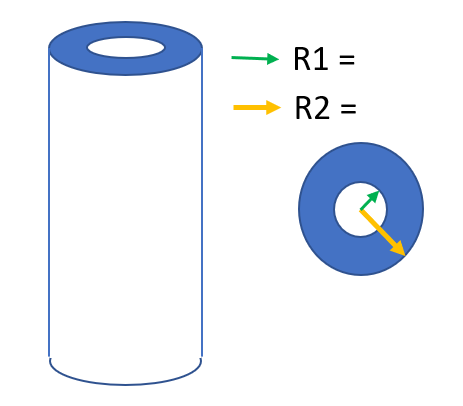
\includegraphics[scale=0.7]{final_7.png}
\end{center}
\end{figure}

Utilizing Ampere's Law, write the equations for the magnitude of the magnetic field (B) for the below conditions. 

\begin{itemize}
\item $r < R_1$?
\item $R_1 < r < R_2$?
\item $r > R_2$?
\end{itemize}

Finally, graph the resulting magnitude of magnetic field as a function of $r$?

\textbf{Question 8 - Extra Credit} (5pts)
Which of Maxwell's Equations can be attributed to Benjamin Franklin?
 

\end{document}
